\chapter{Future Plan and Conclusions}\label{C:con}

This report introduces the use of Neo4j graph databases to model QoS-aware web service compositions. The proposed five algorithms can efficiently create the database, reduce the database, and generate an initial population. The proposed algorithm can automatically construct a relatively good initial population. Our evaluation results have verified the correctness of web service compositions created using our algorithms.

Currently, our proposed method is only able to generate initial populations. In the second part of the project, we will use QoS to calculate global optimisation to find better web service compositions. We may consider using GP to improve initial populations by using mutation and crossover operators.

The first task for future work is to design a fitness function to produce solutions with the smallest possible number of service nodes and with the shortest possible paths from the start node to the end node. The second task for future work is to build QoS-aware compositions and calculate the global optimisation and improve the results. The third task for future work is to analyse and design the evaluation by comparing the performance of our system against the traditional GP approach and other GP approaches.  The Figure 4.1 shows the current working progress. As shown in Figure 4.1, our objectives 1, 2, and 3 have been achieved. The rest of our work is to analyse more preliminary evaluations and start on design work for objectives 4 and 5 early enough to be able to revisit and modify objective 3 if needed.\\

\begin{figure}[h]
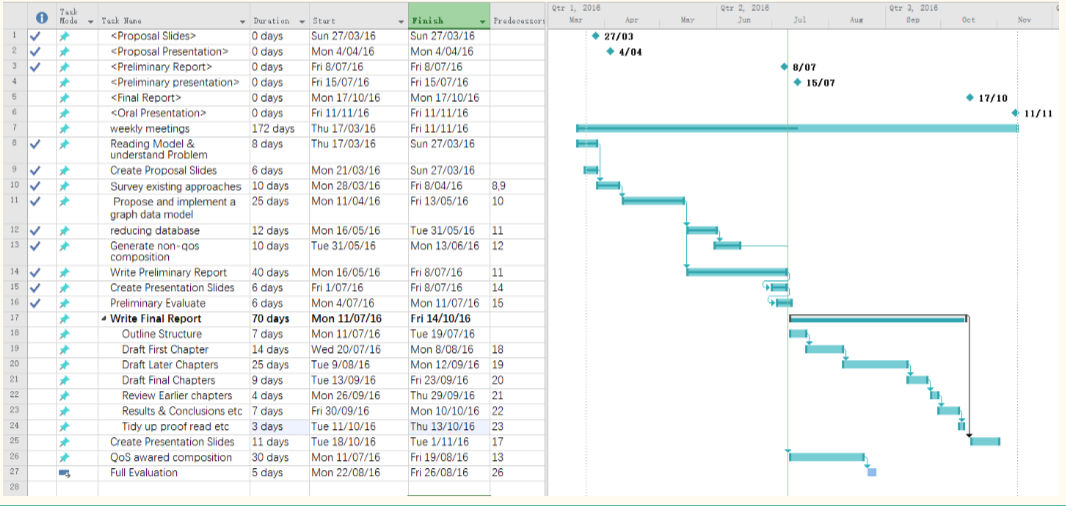
\includegraphics[width=15cm]{ganttChart.png}
\centering
\caption{GANNT CHART}
\end{figure}

